\chapter{Evaluierung}
\label{chap:evaluierung}

Ziel der Evaluierung ist die Überprüfung, ob das entwickelte System die in
Kapitel~\ref{chap:anforderungsanalyse} formulierten Anforderungen erfüllt. Im
Mittelpunkt steht dabei die drahtlose Übertragung, da sie gegenüber der
kabelgebundenen Signalführung die einzige neu eingeführte und zugleich am
wenigsten vorhersagbare Komponente der Signalkette darstellt. Für sie werden
quantitative Messreihen erhoben. Ergänzend wird die elektrische
Leistungsaufnahme einer Leuchtröhre gemessen, da sie den in
Abschnitt~\ref{subsec:elektrische-belastbarkeit} rechnerisch festgelegten
Auslegungswert unmittelbar überprüfbar macht. Die übrigen Anforderungen werden
funktional verifiziert. Die Grenzen der erhobenen Daten sind in
Abschnitt~\ref{sec:grenzen} zusammengefasst.

\section{Evaluierungsziele und Methodik}
\label{sec:evaluierungsziele}

\subsection{Evaluierungsziele}
\label{subsec:evaluierungsziele-ableitung}

Aus den Anforderungen ergeben sich vier quantitativ überprüfbare Ziele. Erstens
muss die Funkstrecke die Steuerdaten mit einer für flüssige Lichtsteuerung
ausreichenden Rate und zeitlichen Konstanz übertragen
(Abschnitt~\ref{subsec:echtzeitverhalten}). Zweitens muss die Verbindung eine
Reichweite erreichen, die typische Bühnenszenarien abdeckt.
In Abschnitt~\ref{subsec:fa-kommunikation} wurden 50 Meter als Mindestreichweite festgelegt. 
Drittens muss die Übertragung auch in
hochfrequenzbelasteten Umgebungen ausreichend zuverlässig bleiben
(Abschnitt~\ref{subsec:zuverlaessigkeit}). Die Messreihen sind entsprechend in
eine Referenzmessung unter Idealbedingungen, zwei Reichweitenmessreihen mit und
ohne Sichtverbindung sowie eine Messreihe unter realer Fremdfunklast gegliedert.
Viertens muss die Leuchtröhre den in
Abschnitt~\ref{subsec:elektrische-belastbarkeit} zugrunde gelegten Betriebsstrom
im Dauerbetrieb einhalten, hierzu dient die Leistungsmessung in
Abschnitt~\ref{sec:leistungsaufnahme}.

\subsection{Messaufbau und Testfirmware}
\label{subsec:messaufbau}

Alle Messreihen wurden mit der in Abschnitt~\ref{sec:testaufbau} beschriebenen
Mess-Firmware auf der Zielhardware erhoben, bestehend aus einer Bridge (ESP32)
als Sender und einer Leuchtröhre (XIAO ESP32-S3) als Empfänger. Der Sender
verwendet nicht eine eigens für den Test geschriebene Übertragungsroutine,
sondern die produktive Klasse \texttt{WirelessDmxController} aus
Abschnitt~\ref{subsec:espnow}. Gemessen wird damit der tatsächlich ausgelieferte
Sendepfad einschließlich Broadcast-Adressierung, Rahmenformat und Kanalzuordnung.

Übertragen werden Pakete mit 80 DMX-Kanälen. Als Nutzdaten dient ein
fortlaufender Sequenzzähler, dessen Wert alle 25\,ms erhöht wird. Ddas entspricht
einer Aktualisierungsrate von 40\,Hz und damit näherungsweise der maximalen
DMX512-Wiederholrate von 44\,Hz \cite{ANSI_E1.11_2024,yang2015real}. Unabhängig
davon wird alle 5\,ms ein Paket ausgesendet, sodass jeder Sequenzwert nominell
fünfmal übertragen wird (Abbildung~\ref{fig:messtakte}). Das feste Sendeintervall
bildet das ungedrosselte Wiederholen der produktiven Bridge nach und macht die
Läufe untereinander vergleichbar. Der Empfänger wertet jedes eingehende Paket
unmittelbar im Empfangs-Callback aus, rekonstruiert aus den Lücken des
Sequenzzählers den Verlust und gibt einmal je Sekunde eine CSV-Zeile mit
Fenster- und Summenkennwerten über die serielle Schnittstelle aus. Die Auswertung
im Callback ist notwendig, weil die Hauptschleife Pakete verwerfen würde, die
zwischen zwei Durchläufen eintreffen.

Für sämtliche Läufe gelten dieselben Randbedingungen. Beide Geräte tragen eine
externe Antenne (Abschnitt~\ref{subsec:funk-antenne}) und senden mit der
voreingestellten Sendeleistung, die im Quelltext nicht verändert wurde.
Alle Aufzeichnungen erfolgten auf WLAN-Kanal~1 und umfassen 300\,s,
was je Lauf rund 12\,000 Sequenzwerten und etwa 60\,000 physisch ausgesendeten
Paketen entspricht. Bei den Reichweitenmessungen standen Sender und Empfänger
unmittelbar auf dem Boden. Diese Aufstellung ist für Funkstrecken ungünstig.
Die im Folgenden ermittelten Reichweiten sind daher als konservative Untergrenze zu verstehen. 
Je Messpunkt wurde ein Lauf aufgezeichnet.

\subsection{Metriken und Bewertungskriterien}
\label{subsec:metriken}

Aufgrund der mehrfachen Aussendung jedes Sequenzwerts ist zwischen zwei
Verlustbegriffen zu unterscheiden, die im Folgenden konsequent getrennt werden:

\begin{description}
  \item[Sequenzverlust] Anteil der Sequenzwerte, von denen keine der
    Kopien empfangen wurde. Nur dieser Verlust wirkt sich auf die Lichtausgabe
    aus, da die Röhre andernfalls den aktuellen Wert erhält.
  \item[Empfangsredundanz] Mittlere Anzahl empfangener Kopien je
    empfangenem Sequenzwert (Maximum: fünf). Sie beschreibt die
    verbleibende Fehlerreserve der Funkstrecke, bevor ein Sequenzverlust
    überhaupt auftreten kann, und reagiert daher deutlich früher auf eine
    Verschlechterung der Verbindung als der Sequenzverlust selbst.
\end{description}

Ergänzend werden die längste zusammenhängende Verlustserie, der Anteil der
Ein-Sekunden-Fenster mit einer solchen Serie sowie das 95.~Perzentil des
fensterbezogenen Sequenzverlusts erfasst. Letzteres beschreibt das schlechte Ende
der Verteilung und zeigt an, wie weit einzelne Sekunden vom Mittelwert abweichen.
Als Maß für die zeitliche Konstanz dient die Standardabweichung des Abstands
aufeinanderfolgender Sequenzwerte (Jitter). Diese Größe ist allerdings nicht
unabhängig vom Verlust: Fällt ein Sequenzwert aus, geht der verdoppelte Abstand
in die Streuung ein, und bereits der Ausfall früher Kopien verschiebt den
Empfangszeitpunkt um bis zu 20\,ms. Bei niedrigen Verlustraten misst der Jitter
daher die Schwankung des Medienzugriffs, bei hohen Verlustraten gibt er
überwiegend die Verluststatistik wieder. Er wird im Folgenden nur im
erstgenannten Fall als eigenständiger Befund herangezogen.

Das Bewertungskriterium für Verluste folgt aus dem in
Abschnitt~\ref{subsec:zuverlaessigkeit} festgelegten Verhalten bei Ausfällen: Die
Röhre hält den zuletzt empfangenen Lichtzustand. Ein Verlust äußert sich damit
nicht als Dunkelphase, sondern als verlängerte Standzeit des vorherigen Zustands.
Dabei ist zwischen der Gesamtstandzeit und der durch den Verlust verursachten
Verlängerung zu unterscheiden. Die folgenden Tabellen weisen unter
„max.\ Ausfall“ stets die Verlängerung aus.

Ein einzelner verlorener Sequenzwert verlängert die Standzeit um 25\,ms, die
Gesamtstandzeit steigt damit auf 50\,ms. Sie überschreitet die 41,7\,ms, die der
in Abschnitt~\ref{subsec:echtzeitverhalten} angestrebten
Bewegungswahrnehmungsschwelle von 24\,Hz entsprechen, damit geringfügig. Da die
Verlängerung selbst mit 25\,ms deutlich unterhalb dieser Schwelle bleibt und ein
Einzelverlust bei bewegten Effekten unauffällig ist, wird er im Folgenden als
tolerabel eingestuft. Ab zwei aufeinanderfolgenden verlorenen Sequenzwerten
überschreiten sowohl die Verlängerung (50\,ms) als auch die Gesamtstandzeit
(75\,ms) die Schwelle, ab drei Verlusten (75\,ms Verlängerung) auch die
konservativere Schwelle von 15\,Hz
\cite{fujii2018,ramunae2025}. Als Kriterium wird daher nicht allein die mittlere
Verlustrate herangezogen, sondern zusätzlich der Anteil der Sekundenfenster mit
einer Verlustserie von mindestens zwei Sequenzwerten. Er ist in den folgenden
Tabellen als „Fenster ab 50\,ms“ ausgewiesen.

\subsection{Reproduzierbarkeit und Grenzen der Instrumentierung}
\label{subsec:messgrenzen}

Die Aufzeichnung erfolgt hostseitig zeitbegrenzt über ein Skript, das die serielle
Ausgabe unverändert in eine CSV-Datei schreibt. Die Rohdaten werden nicht
nachbearbeitet. Ssämtliche Tabellen und Abbildungen dieses Kapitels werden
deterministisch aus ihnen erzeugt. Verworfen werden lediglich die Zeilen vor dem
Eintreffen des ersten Pakets, für die die Firmware definitionsgemäß 100\,\%
Verlust meldet und die andernfalls jede Fensterstatistik verfälschen würden. 
Im vorliegenden Datensatz betrifft dies je Lauf genau eine Zeile. Rohdaten,
Mess-Firmware und Auswertungsskript sind gemeinsam mit der Anwendungsfirmware
unter \url{https://github.com/nichtrami/led_tube} veröffentlicht. Die Tabellen
und Abbildungen werden bei jeder Auswertung neu erzeugt und nicht separat
versioniert, sodass sie stets dem Stand der Rohdaten entsprechen.

Drei Eigenschaften der Instrumentierung begrenzen die Aussagekraft der
Messgrößen. Erstens ist der übertragene Sequenzzähler acht Bit breit,
Verlustserien ab 256 Sequenzwerten entsprechend 6,4\,s würden modulo 256
aliasiert und dadurch unterzählt. Die längste beobachtete Serie umfasst 38 Werte,
sodass dieser Fall in keiner Messreihe eintritt. Zweitens leitet der Empfänger
die erwartete Anzahl Sequenzwerte aus dem empfangenen Zähler ab. Ein
ausbleibender Sendevorgang der Bridge ist damit von einem Verlust auf der
Funkstrecke nicht zu unterscheiden. Drittens wertet der Sender den Rückgabewert
des Sendeaufrufs nicht aus, sodass auch senderseitig nicht protokolliert wird, ob
ein Paket überhaupt abgesetzt werden konnte. Die beiden letztgenannten Punkte
sind für die Deutung der Störfestigkeitsmessung in
Abschnitt~\ref{sec:stoerfestigkeit} von Bedeutung.

Eine weitere Einschränkung betrifft die Erfassung der Empfangsfeldstärke (RSSI). Der
ESP-NOW-Empfangs-Callback stellt diesen Wert nicht bereit. Er wird deshalb über
einen parallel betriebenen Promiscuous-Modus ermittelt, der die Feldstärke des
jeweils zuletzt auf dem Kanal empfangenen Datenpakets speichert. Dieses Paket
stammt nicht zwingend vom Sender des Systems. Die aufgezeichneten Werte sind
folglich kein Maß für den Pfadverlust der Nutzstrecke, was die Messdaten
unmittelbar belegen: Über 0\,m wird im Mittel $-81{,}6$\,dBm ausgewiesen, über
200\,m dagegen $-63{,}4$\,dBm und damit ein höherer Pegel bei größerer
Entfernung. Der RSSI wird daher im Folgenden ausschließlich als grober Indikator
der Fremdsenderaktivität auf dem Kanal verwendet und nicht zur Bewertung der
Reichweite herangezogen.

\section{Funktionale Verifikation}
\label{sec:funktionale-tests}

Die funktionalen Anforderungen wurden durch Erprobung am aufgebauten System
überprüft. Sie sind qualitativer Natur und liefern keine Messgrößen.

Im Standalone-Modus arbeitet die Leuchtröhre ohne Bridge und ohne jede
Funkkommunikation. Die über das Bedienmenü gewählte Farbe und der gewählte Effekt
werden unmittelbar auf den LED-Strip angewendet. Sämtliche Konfigurationsparameter
Betriebsmodus, DMX-Adresse, Kanal, Farbe und Effekt werden persistent
gespeichert und nach einem Neustart selbsttätig wiederhergestellt, sodass nach
einer Spannungsunterbrechung kein erneutes Einrichten erforderlich ist. Die
Umschaltung zwischen den Betriebsmodi ist im laufenden Betrieb möglich. Das Menü
blendet dabei nur die für den aktiven Modus relevanten Einträge ein.

Im drahtlosen Modus extrahiert die Bridge die zur konfigurierten Startadresse
gehörenden Kanäle aus dem eingehenden DMX-Universum und überträgt sie an die
Röhren. Die Röhren setzen die empfangenen Kanalwerte über den vollen Wertebereich
in Helligkeit und Farbe um. Der erste der vier belegten Kanäle wählt den Effekt.
Da adressabhängig aus demselben Broadcast unterschiedliche Abschnitte gelesen
werden, lassen sich mehrere Röhren mit unterschiedlichen DMX-Adressen gleichzeitig
und unabhängig ansteuern. Erprobt wurde dies mit acht gleichzeitig an einer
Bridge betriebenen Leuchtröhren, die über unterschiedliche Startadressen
unabhängig voneinander angesteuert wurden. Das entspricht 40\,\% der in
Abschnitt~\ref{subsec:fa-kommunikation} festgelegten Ausbaugröße von 20 Röhren.
Da die Bridge unabhängig von der Empfängerzahl denselben Broadcast aussendet,
wächst die Funklast mit weiteren Röhren nicht an. Die volle Ausbaugröße wurde
jedoch nicht erprobt (Abschnitt~\ref{sec:grenzen}). Ob die Röhren dabei
gleichzeitig reagieren, wird in Abschnitt~\ref{sec:gleichzeitigkeit} gesondert
untersucht.

Der Signaleingang der Bridge wurde in beiden vorgesehenen Varianten überprüft.
Neben dem kabelgebundenen DMX-Eingang (Abschnitt~\ref{subsec:dmx-eingang}) nimmt
die Bridge ein Art-Net-Universum über die Ethernet-Schnittstelle entgegen
(Abschnitt~\ref{subsec:artnet-eingang}) und überführt es in dasselbe interne
Format. Die nachgelagerte Verarbeitung und die Funkübertragung bleiben dadurch
unverändert. Die Lichtausgabe an den Röhren ist zwischen beiden Eingängen nicht
zu unterscheiden.

Im Master-Modus erzeugt die Bridge den Lichtzustand selbst
(Abschnitt~\ref{subsec:bridge-modi}). Sie durchläuft ohne externes Steuersignal
eine Folge von Farben und Effekten, deren Tempo über die im Bedienmenü
eingestellte Schlagzahl vorgegeben wird, und überträgt das Ergebnis über
dieselbe Funkschnittstelle. Da alle Röhren denselben Broadcast empfangen,
entsteht dabei ein über sämtliche Geräte hinweg einheitliches Lichtbild, ohne
dass eine externe Lichtsteuerung angeschlossen ist.

\section{Übertragungsverhalten unter Idealbedingungen}
\label{sec:idealbedingungen}

Als Referenz dienen die beiden kürzesten Messpunkte der Reichweitenreihe bei
0\,m und 10\,m Abstand mit freier Sicht zwischen den Geräten. In beiden Läufen
wurde kein einziger Sequenzwert verloren: Von jeweils 11\,992 erwarteten
Sequenzen kamen alle an, sämtliche Sekundenfenster waren verlustfrei.

Aus dem Ausbleiben eines Ereignisses lässt sich keine Verlustrate von exakt null
ableiten. Nach der Regel der Drei ergibt sich aus null Verlusten bei
$n = 11\,992$ Beobachtungen eine obere Grenze des 95\,\%-Konfidenzintervalls von
$3/n \approx 0{,}025\,\%$ Über beide Läufe zusammen ($n = 23\,984$) entsprechend
$0{,}013\,\%$. Zur Einordnung: Selbst wenn jeder einzelne Verlust bereits eine
sichtbare Verlustserie bildete, entspräche diese obere Schranke bei 40
Sequenzwerten je Sekunde höchstens einem Ereignis alle drei Minuten. Die
tatsächliche Verlustrate unter Idealbedingungen liegt darunter.

Die Empfangsredundanz beträgt 5,00 bzw.\ 4,99 Kopien je Sequenzwert, die
Fehlerreserve der Strecke ist also praktisch vollständig vorhanden. Der mittlere
Abstand aufeinanderfolgender Sequenzwerte entspricht mit 25,00\,ms exakt der
Sollrate. Der Jitter liegt bei 4,1\,ms bzw.\ 6,2\,ms. Da er damit deutlich
unterhalb des Frameabstands von 25\,ms bleibt, entsteht keine wahrnehmbare
Unregelmäßigkeit der Lichtausgabe. Die Anforderung an Aktualisierungsrate und
zeitliche Konstanz aus Abschnitt~\ref{subsec:echtzeitverhalten} ist auf der
Funkstrecke somit erfüllt.

\section{Gleichzeitigkeit der Lichtausgabe}
\label{sec:gleichzeitigkeit}

Die bisherigen Messreihen beschreiben die Übertragung zu einer einzelnen Röhre.
Für den praktischen Einsatz ist darüber hinaus entscheidend, ob alle Röhren
denselben Lichtzustand zum selben Zeitpunkt anzeigen. Ein sichtbarer Versatz
zwischen benachbarten Leuchten würde ein zusammenhängendes Lichtbild zerstören,
und zwar unabhängig davon, wie gering die Verzögerung gegenüber der Lichtsteuerung
insgesamt ausfällt. Die Broadcast-Topologie legt nahe, dass ein solcher Versatz
nicht auftritt, da sämtliche Röhren dasselbe Paket empfangen und keine
gerätespezifische Adressierung durchlaufen (Abschnitt~\ref{subsec:espnow}). Ein
Nachweis folgt daraus jedoch nicht.

Zur Überprüfung wurden acht gleichzeitig betriebene Leuchtröhren gemeinsam
gefilmt, während der Lichtzustand sprunghaft gewechselt wurde. Die Aufnahme
erfolgte als Zeitlupenvideo mit 120~Bildern je Sekunde, sodass aufeinanderfolgende
Einzelbilder einen zeitlichen Abstand von rund 8,4\,ms besitzen. Ein Versatz
zwischen zwei Röhren wäre damit als Einzelbild erkennbar, in dem ein Teil der
Röhren bereits umgeschaltet hat und der andere noch den vorherigen Zustand zeigt.

In der Auswertung der Aufnahme wechseln sämtliche Röhren innerhalb desselben
Einzelbildes. Ein Versatz zwischen den Geräten ist mit diesem Verfahren somit
nicht nachweisbar. Die Abweichung liegt unterhalb der zeitlichen Auflösung von
8,4\,ms und damit weit unterhalb der in
Abschnitt~\ref{subsec:echtzeitverhalten} angesetzten Wahrnehmungsschwelle von
41,7\,ms. Die Annahme, dass die Broadcast-Übertragung alle Empfänger innerhalb
desselben Übertragungsfensters erreicht, ist damit für den erprobten Aufbau
bestätigt.

\section{Reichweite}
\label{sec:reichweitentest}

Die Reichweitenmessungen wurden an den Ostplatz-Arkaden in Leipzig durchgeführt,
einem Straßenzug in bebautem Gelände mit seitlicher Bebauung sowie Passanten- und
Fahrzeugverkehr. Der Abstand zwischen Bridge und Leuchtröhre wurde schrittweise
erhöht, bei ansonsten unverändertem Aufbau, gleichem Kanal und gleicher Messdauer
von 300\,s je Messpunkt.

Aufgezeichnet wurden zwei Messreihen. In der ersten bestand eine durchgehende
Sichtverbindung entlang der Straßenachse. In der zweiten stand der Empfänger an
jedem Messpunkt rund 50\,cm mittig hinter einer massiven, etwa 1\,m breiten
Stahlbetonstütze und war damit vollständig verdeckt. Die Position des Senders und
alle übrigen Parameter blieben unverändert. Die zweite Reihe bildet damit den in
Innenräumen und Hallen typischen Fall ab, in dem die direkte Sichtlinie durch ein
massives Bauteil unterbrochen ist und die Strecke nur über Beugung und Reflexionen
überbrückt wird.

\subsection{Messreihe mit Sichtverbindung}
\label{subsec:reichweite-los}

Tabelle~\ref{tab:range-summary} fasst die Ergebnisse zusammen,
Abbildung~\ref{fig:range-distanz} stellt Sequenzverlust und Empfangsredundanz
über der Distanz dar.


\begin{table}[htbp]
  \centering
  \small
  \begin{tabular}{lrrrrrrr}
    \toprule
    Messpunkt & Verlust & Fenster p95 & Kopien & Jitter & max. Ausfall & Fenster & RSSI \\
    & [\%] & [\%] & je Seq. & [ms] & [ms] & ab 50 ms [\%] & [dBm] \\
    \midrule
    0 m & 0 & 0 & 5,00 & 4,14 & 0 & 0 & $-$81,64 \\
    10 m & 0 & 0 & 4,99 & 6,16 & 0 & 0 & $-$82,39 \\
    50 m & 0,06 & 0 & 4,62 & 5,82 & 25 & 0 & $-$81,50 \\
    100 m & 0,09 & 0 & 4,43 & 6,62 & 75 & 0,33 & $-$82,85 \\
    150 m & 2,81 & 12,22 & 3,39 & 8,71 & 275 & 8,67 & $-$79,27 \\
    200 m & 10,61 & 31,72 & 2,38 & 14,94 & 425 & 40,67 & $-$63,44 \\
    \bottomrule
\end{tabular}
\caption{Reichweitenmessung (mit Sichtverbindung)}
  \label{tab:range-summary}
\end{table}


\begin{figure}[htbp]
  \centering
  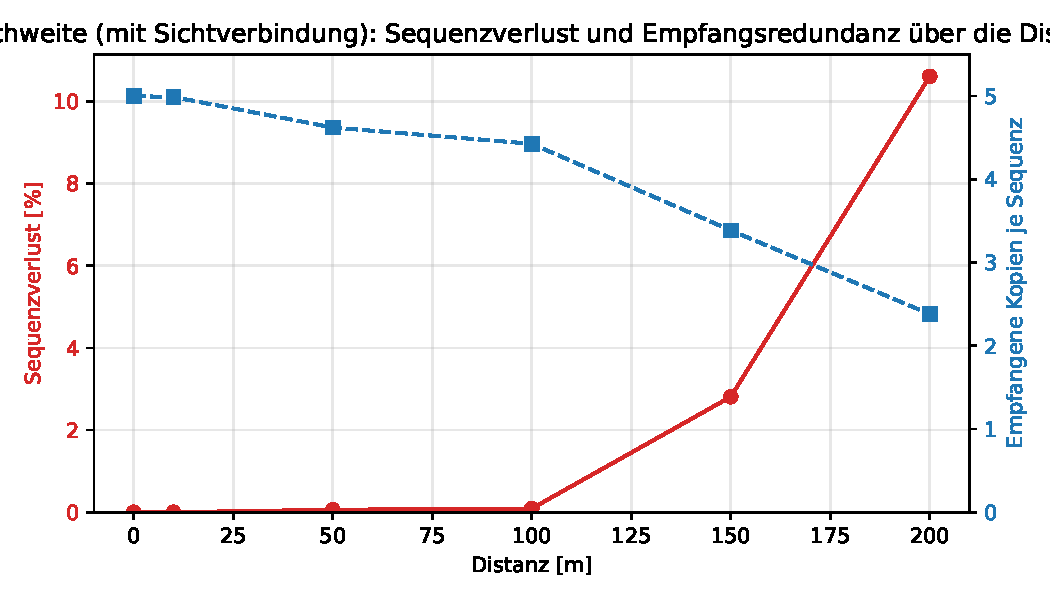
\includegraphics[width=\linewidth]{../test_programs/results/analysis/figures/range_distance.pdf}
  \caption{Sequenzverlust und Empfangsredundanz in Abhängigkeit der Distanz bei
    freier Sichtverbindung. Die Redundanz nimmt bereits ab, während der
    Sequenzverlust noch nahezu bei null liegt.}
  \label{fig:range-distanz}
\end{figure}

Bis einschließlich 100\,m ist die Übertragung praktisch verlustfrei: Bei 50\,m
gingen 7 von 11\,992 Sequenzwerten verloren (0,06\,\%), bei 100\,m 11 von 11\,992
(0,09\,\%). Die längste zusammenhängende Verlustserie beträgt dabei 25\,ms
respektive 75\,ms, und der Anteil der Sekundenfenster mit einer für die
Bewegungswahrnehmung relevanten Verlustserie liegt bei 0\,\% respektive
0,33\,\%. In diesem Bereich ist die Funkstrecke für die Lichtausgabe damit
unauffällig.

Zwischen 100\,m und 150\,m tritt ein deutlicher Übergang auf. Der Sequenzverlust
steigt auf 2,81\,\%, der Anteil vollständig verlustfreier Sekundenfenster fällt
von 97,0\,\% auf 61,0\,\%, und in 8,67\,\% der Fenster wird die Standzeit um
mindestens 50\,ms verlängert. Ebenso deutlich zeigt sich der Übergang am
95.~Perzentil des fensterbezogenen Verlusts: Bis 100\,m liegt es bei 0\,\%, bei
150\,m bereits bei 12,22\,\%. Bei 200\,m liegt der Verlust bei 10,61\,\%, nur
noch 8,67\,\% der Fenster sind verlustfrei, 40,67\,\% enthalten eine sichtbar
relevante Verlustserie, das 95.~Perzentil erreicht 31,72\,\% und die längste
Verlängerung der Standzeit 425\,ms. Der mittlere Abstand empfangener
Sequenzwerte wächst dabei von 25,0\,ms auf 28,5\,ms die effektive
Aktualisierungsrate sinkt damit von 40\,Hz auf rund 35\,Hz. Der gleichzeitige
Anstieg des Jitters von 6,6\,ms auf 14,9\,ms ist dabei keine unabhängige
Beobachtung, sondern ergibt sich aus den Verlustlücken selbst
(Abschnitt~\ref{subsec:metriken}).

Anders als der Verlust verläuft die Empfangsredundanz über die gesamte Messreihe
streng monoton: 5,00 (0\,m), 4,99 (10\,m), 4,62 (50\,m), 4,43 (100\,m), 3,39
(150\,m) und 2,38 Kopien je Sequenzwert bei 200\,m. Sie ist damit die
aussagekräftigere Größe zur Bewertung der Reichweite, denn sie zeigt den Rückgang
der Fehlerreserve bereits an, während der Sequenzverlust noch nahezu bei null
liegt.
Zugleich erklärt sie den flachen Verlauf des Verlusts bis 100\,m: Solange
mindestens eine der fünf Kopien eintrifft, bleibt der Sequenzwert vollständig
erhalten. Erst wenn die Redundanz gegen eins sinkt, schlägt jede weitere
Verschlechterung unmittelbar auf die Lichtausgabe durch.

Die zeitliche Auflösung der Läufe in Abbildung~\ref{fig:range-zeit} zeigt, dass
die Verluste bei den großen Distanzen nicht auf einzelne Störereignisse
zurückgehen, sondern über den gesamten Lauf verteilt auftreten: Im Lauf über
200\,m liegt der minutenweise gemittelte Verlust zwischen 6,41\,\% und 16,40\,\%,
im Lauf über 150\,m zwischen 2,14\,\% und 3,61\,\%. Maßgeblich für das
Verlustniveau ist damit die mit der Distanz abnehmende Reserve der Strecke und
nicht eine kurzzeitige Abschattung durch Passanten oder Fahrzeuge. Die
verbleibende Schwankung zwischen den Minuten
ist mit einem Faktor von 2,6 im 200-m-Lauf allerdings erheblich und zeigt, dass
die Umgebung auch bei freier Sicht zeitveränderlich auf die Verbindung wirkt.

Dazu passt ein Nebenbefund: Für den Lauf über 200\,m weist die Aufzeichnung einen
mittleren Fremdpegel von $-63{,}4$\,dBm aus, gegenüber rund $-80$\,dBm an allen
übrigen Messpunkten. Da dieser Wert die Aktivität fremder Sender auf dem Kanal
beschreibt und nicht den Pegel der Nutzstrecke
(Abschnitt~\ref{subsec:messgrenzen}), deutet er auf eine erhöhte Kanalbelegung
während dieses Laufs hin. Deren Beitrag lässt sich vom Einfluss der Distanz nicht
trennen.

\begin{figure}[htbp]
  \centering
  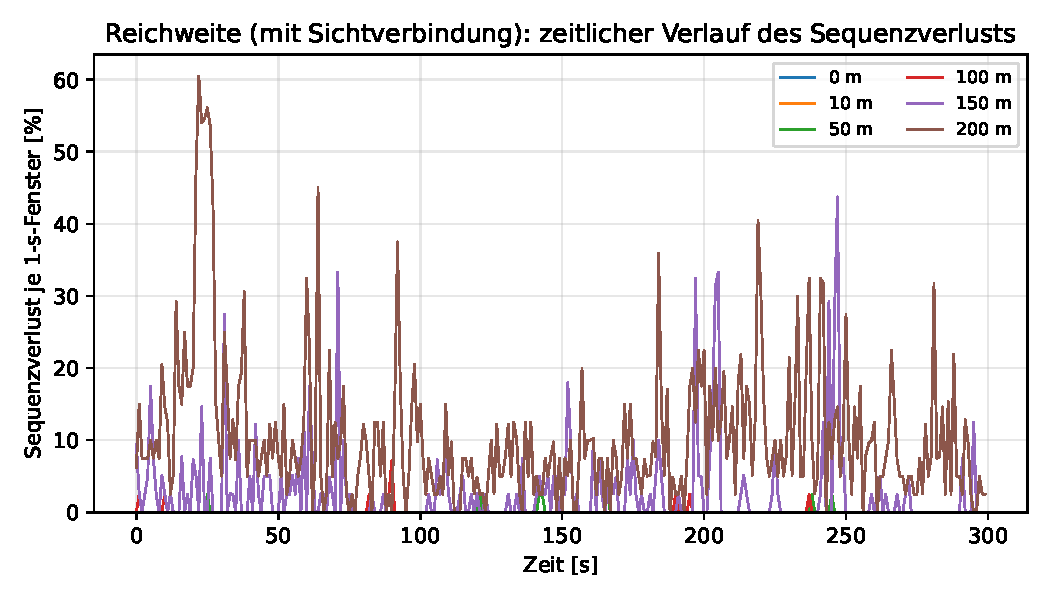
\includegraphics[width=\linewidth]{../test_programs/results/analysis/figures/range_timeseries.pdf}
  \caption{Zeitlicher Verlauf des Sequenzverlusts je Messpunkt bei freier
    Sichtverbindung. Bei 150\,m und 200\,m verteilen sich die Verluste über den
    gesamten Lauf.}
  \label{fig:range-zeit}
\end{figure}

\subsection{Messreihe ohne Sichtverbindung}
\label{subsec:reichweite-verdeckt}

Tabelle~\ref{tab:range-hidden-summary} und Abbildung~\ref{fig:range-hidden-distanz}
zeigen dieselbe Auswertung für den vollständig verdeckten Empfänger.

% Requires \usepackage{booktabs}; otherwise replace \toprule etc. with \hline.
\begin{table}[htbp]
  \centering
  \small
  \begin{tabular}{lrrrrrrr}
    \toprule
    Messpunkt & Verlust & Fenster p95 & Kopien & Jitter & max. Ausfall & Fenster & RSSI \\
    & [\%] & [\%] & je Seq. & [ms] & [ms] & ab 50 ms [\%] & [dBm] \\
    \midrule
    10 m & 0,48 & 0 & 4,80 & 6,96 & 75 & 1,67 & $-$81,23 \\
    50 m & 2,08 & 10,08 & 3,57 & 9,23 & 225 & 7,33 & $-$77,85 \\
    100 m & 10,86 & 36,64 & 2,72 & 16,45 & 575 & 37 & $-$82,97 \\
    150 m & 27,18 & 60,80 & 1,87 & 26,59 & 700 & 80 & $-$48,70 \\
    200 m & 36,29 & 63,67 & 1,61 & 32,12 & 950 & 95,67 & $-$77,39 \\
    \bottomrule
\end{tabular}
\caption{Reichweitenmessung (ohne Sichtverbindung)}
  \label{tab:range-hidden-summary}
\end{table}


\begin{figure}[htbp]
  \centering
  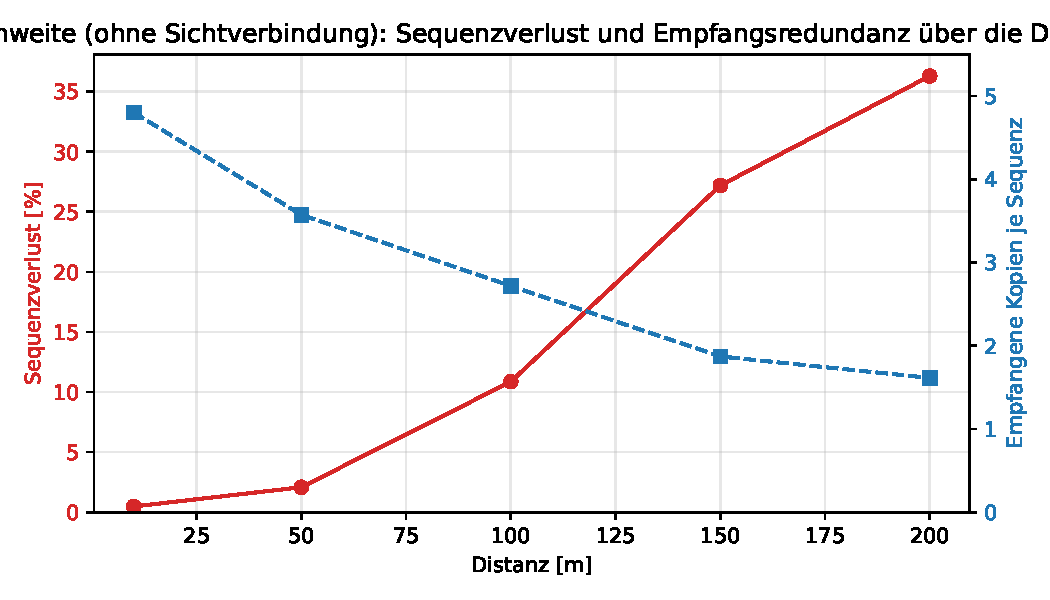
\includegraphics[width=\linewidth]{../test_programs/results/analysis/figures/range_hidden_distance.pdf}
  \caption{Sequenzverlust und Empfangsredundanz über der Distanz bei verdecktem
    Empfänger (rund 50\,cm hinter einer 1\,m breiten Stahlbetonstütze).}
  \label{fig:range-hidden-distanz}
\end{figure}

Bei 10\,m bleibt die Verbindung nahezu unbeeinträchtigt: Der Sequenzverlust
beträgt 0,48\,\%, die Redundanz 4,80 Kopien je Sequenzwert. Die Verluste sind
zudem auf ein einzelnes Ereignis in der dritten Minute konzentriert ein
Sekundenfenster weist 30,91\,\% Verlust auf, während 97,67\,\% aller Fenster
vollständig verlustfrei sind. Auf kurzer Distanz genügt die Beugung um die Stütze
also, um die Strecke zu tragen.

Mit zunehmender Entfernung verschlechtert sich die Verbindung deutlich schneller
als in der Sichtreihe. Bei 50\,m liegt der Verlust bei 2,08\,\% und die Redundanz
bei 3,57. 7,33\,\% der Sekundenfenster enthalten eine Verlustserie ab 50\,ms, die
längste Verlängerung der Standzeit beträgt 225\,ms. Bei 100\,m steigt der Verlust
auf 10,86\,\%, die Redundanz fällt auf 2,72, und in 37,00\,\% der Fenster wird die
Wahrnehmungsschwelle überschritten. Bei 150\,m gehen bereits 27,18\,\% der
Sequenzwerte verloren, die Redundanz beträgt noch 1,87 Kopien, 80,00\,\% der
Fenster überschreiten die Schwelle und lediglich 0,67\,\% zwei von 300
sind vollständig verlustfrei. Bei 200\,m schließlich ist die Strecke nicht
mehr sinnvoll nutzbar: 36,29\,\% der Sequenzwerte gehen verloren, die Redundanz
sinkt auf 1,61 Kopien in einzelnen Fenstern auf exakt 1,00, \emph{kein
einziges} Sekundenfenster ist verlustfrei, 95,67\,\% der Fenster überschreiten
die 50-ms-Schwelle und die längste Verlängerung der Standzeit erreicht 950\,ms.
Der mittlere Abstand empfangener Sequenzwerte wächst auf 42,3\,ms, was einer
effektiven Aktualisierungsrate von rund 24\,Hz entspricht. Die Übertragung
unterschreitet damit erstmals die in Abschnitt~\ref{subsec:echtzeitverhalten}
angestrebte Aktualisierungsrate.

Auch hier zeigt die zeitliche Auflösung (Abbildung~\ref{fig:range-hidden-zeit})
eine zusätzliche Variabilität der Umgebung: Im Lauf über 100\,m liegt der Verlust
in den ersten drei Minuten zwischen 12,63\,\% und 19,08\,\%, in den letzten
beiden dagegen nur bei 2,51\,\% und 3,91\,\%. Eine kontrollierte Zuordnung zu
konkreten Umgebungsereignissen ist aus den Daten nicht möglich. Die Beobachtung
belegt jedoch, dass auf verdeckten Strecken neben der Distanz auch
zeitveränderliche Einflüsse eine erhebliche Rolle spielen. Der Lauf über 150\,m
zeigt umgekehrt keinen solchen Verlauf: Sein minutenweiser Verlust bleibt
durchgehend zwischen 22,58\,\% und 29,19\,\%, die Strecke ist über die gesamte
Messdauer gleichmäßig schlecht. Für diesen Messpunkt weist die Aufzeichnung
allerdings einen mittleren Fremdpegel von $-48{,}7$\,dBm aus und damit den
höchsten Wert aller Läufe. Wie beim 200-m-Lauf der Sichtreihe ist eine erhöhte
Kanalbelegung als zusätzlicher Einfluss nicht auszuschließen
(Abschnitt~\ref{subsec:messgrenzen}).

\begin{figure}[htbp]
  \centering
  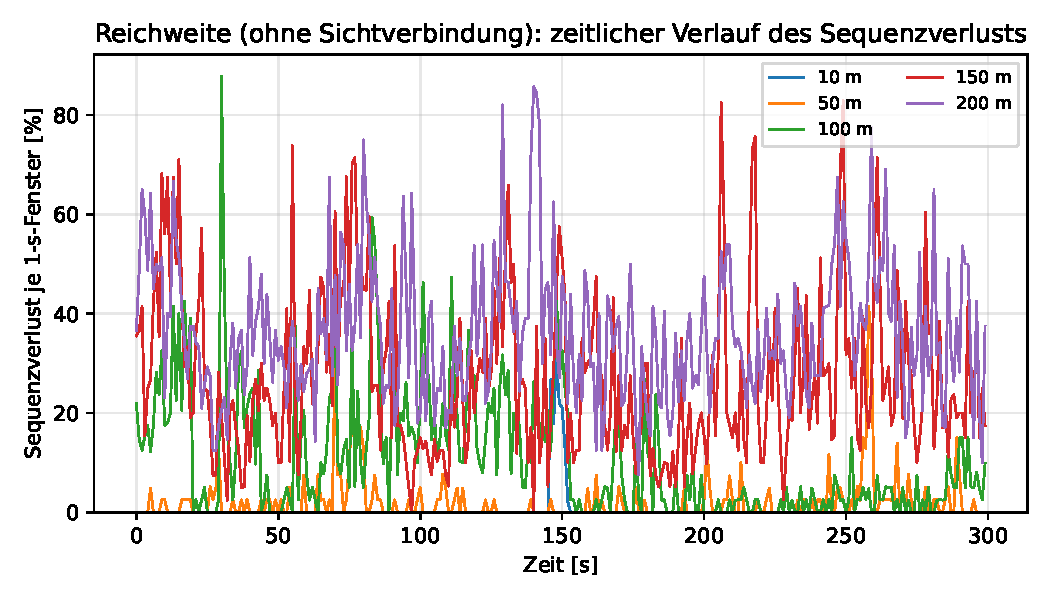
\includegraphics[width=\linewidth]{../test_programs/results/analysis/figures/range_hidden_timeseries.pdf}
  \caption{Zeitlicher Verlauf des Sequenzverlusts je Messpunkt bei verdecktem
    Empfänger. Der Lauf über 100\,m verbessert sich in der zweiten Hälfte
    deutlich.}
  \label{fig:range-hidden-zeit}
\end{figure}

\subsection{Vergleich und Bewertung}
\label{subsec:reichweite-bewertung}

Der Vergleich beider Reihen bei gleicher Distanz quantifiziert die Wirkung der
Abschattung. Bei 50\,m steigt der Verlust von 0,06\,\% auf 2,08\,\% und die
Redundanz sinkt von 4,62 auf 3,57 Kopien. Bei 100\,m stehen 0,09\,\% und 4,43
Kopien einem Verlust von 10,86\,\% bei 2,72 Kopien gegenüber. Das verdeckte
Verhalten bei 100\,m entspricht dabei praktisch dem Verhalten der Sichtreihe bei
200\,m (10,61\,\%, 2,38 Kopien).

Die Abschattung wirkt wie ein näherungsweise konstanter Dämpfungszuschlag. Da ein
solcher Zuschlag im logarithmischen Pfadverlustmodell einem konstanten Faktor der
Distanz entspricht, lässt sich die Wirkung als äquivalente Sichtdistanz
ausdrücken. Vergleicht man die verdeckten Messpunkte anhand der Empfangsredundanz
mit der interpolierten Sichtreihe, ergeben sich Faktoren von etwa 2,8 bei 50\,m,
1,8 bei 100\,m und 1,5 bei 150\,m. Als Faustregel lässt sich daraus ableiten,
dass die vollständige Abschattung durch eine Stahlbetonstütze etwa die Hälfte der
nutzbaren Distanz kostet. Angesichts eines einzelnen Laufs je Messpunkt und der
Streuung zwischen den ermittelten Faktoren ist dieser Wert als Größenordnung und
nicht als belastbarer Zahlenwert zu verstehen.

Für die praktische Bewertung ist die in Abschnitt~\ref{subsec:fa-kommunikation}
festgelegte Mindestreichweite von 50\,m maßgeblich. Mit Sichtverbindung wird
diese Anforderung deutlich übertroffen: Bei 50\,m ist die Übertragung mit
0,06\,\% Verlust und ohne ein einziges kritisches Sekundenfenster faktisch
fehlerfrei, und auch bei 100\,m bleibt dieses Niveau erhalten. Ohne
Sichtverbindung wird die Mindestreichweite ebenfalls erreicht, jedoch mit
sichtbar geringerer Reserve: Bei 2,08\,\% Verlust und 7,33\,\% kritischen Fenstern
ist im Mittel etwa alle 14\,s mit einer verlängerten Standzeit von mindestens
50\,ms zu rechnen. Für die Betriebsplanung folgt daraus die Empfehlung, mit
Sichtverbindung bis etwa 100\,m und ohne Sichtverbindung bis etwa 50\,m zu
projektieren. Jenseits von 150\,m (Sicht) beziehungsweise 100\,m (verdeckt) ist
der Betrieb zwar noch möglich, aber nicht mehr zuverlässig planbar.

\section{Verhalten in hochfrequenzbelasteter Umgebung}
\label{sec:stoerfestigkeit}

Zur Beurteilung der Störfestigkeit wurden zwei Läufe im Lesesaal einer Bibliothek
aufgezeichnet. Sender und Empfänger standen dabei rund 50\,m voneinander
entfernt, wobei die direkte Sichtlinie durch hölzernes Mobiliar unterbrochen war.
Die Messung fand damit genau an der in Abschnitt~\ref{subsec:fa-kommunikation}
geforderten Mindestreichweite statt. Positionen von Sender und Empfänger,
Abstand, Kanal und Firmwarestand blieben zwischen beiden Läufen unverändert
verändert wurde
ausschließlich die Umgebung: Der erste Lauf fand zur Stoßzeit bei hoher
Personendichte und entsprechend vielen aktiven WLAN- und Bluetooth-Geräten statt,
der zweite zur Nebenzeit bei nahezu leerem Lesesaal. Es handelt sich damit um eine
Feldmessung mit realistischer, aber nicht kontrollierter Störlast.
Tabelle~\ref{tab:interference-summary} zeigt die Ergebnisse,
Abbildung~\ref{fig:stoerung-zeit} den zeitlichen Verlauf.

% Requires \usepackage{booktabs}; otherwise replace \toprule etc. with \hline.
\begin{table}[htbp]
  \centering
  \small
  \begin{tabular}{lrrrrrrr}
    \toprule
    Szenario & Verlust & Fenster p95 & Kopien & Jitter & max. Ausfall & Fenster & RSSI \\
    & [\%] & [\%] & je Seq. & [ms] & [ms] & ab 50 ms [\%] & [dBm] \\
    \midrule
    Nebenzeit & 0,01 & 0 & 4,57 & 6,47 & 25 & 0 & $-$83,72 \\
    Stoßzeit & 0,51 & 2,50 & 3,83 & 8,45 & 750 & 0,33 & $-$84,02 \\
    \bottomrule
\end{tabular}
\caption{Messergebnisse Störfestigkeit}
  \label{tab:interference-summary}
\end{table}


\begin{figure}[htbp]
  \centering
  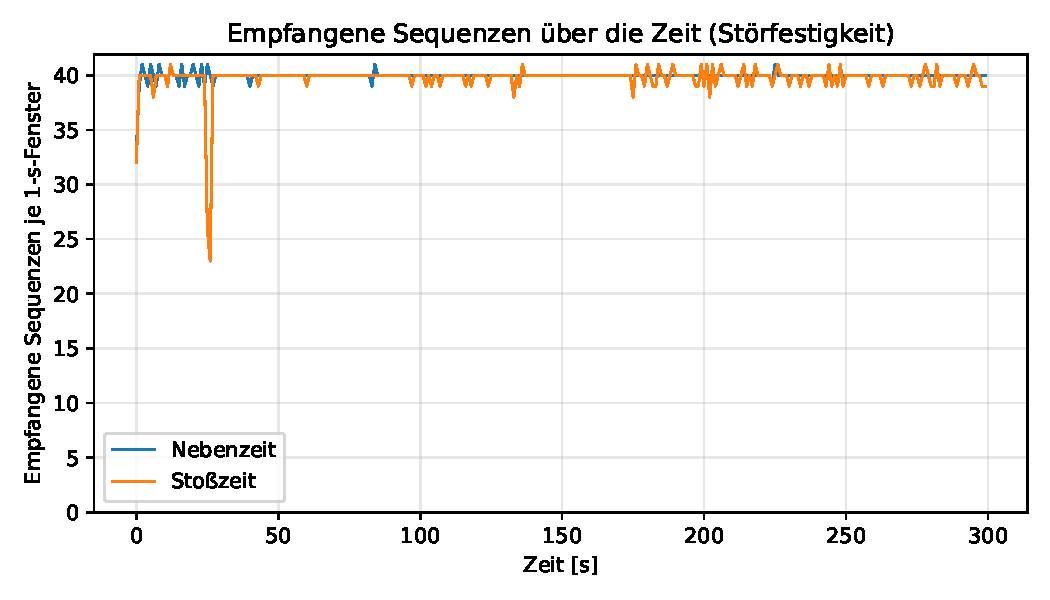
\includegraphics[width=\linewidth]{../test_programs/results/analysis/figures/interference_timeseries.pdf}
  \caption{Empfangene Sequenzen je Sekunde zur Stoßzeit und zur Nebenzeit. Der
    Sollwert beträgt 40 Sequenzen je Sekunde.}
  \label{fig:stoerung-zeit}
\end{figure}

Zur Nebenzeit ist die Übertragung nahezu fehlerfrei: Ein einziger von 11\,992
Sequenzwerten geht verloren (0,01\,\%), 99,67\,\% der Sekundenfenster sind
vollständig verlustfrei und die längste Verlängerung der Standzeit beträgt
25\,ms. Zur Stoßzeit
steigt der Sequenzverlust auf 0,51\,\% (61 von 11\,991), der Anteil verlustfreier
Fenster sinkt auf 89,67\,\% und der Jitter wächst von 6,5\,ms auf 8,5\,ms. Die
Empfangsredundanz geht von 4,57 auf 3,83 Kopien je Sequenzwert zurück. Die
Fehlerreserve der Strecke verringert sich also messbar, bleibt aber mit fast vier
von fünf Kopien komfortabel erhalten.

Der Wert zur Nebenzeit ordnet zugleich den Aufbau ein: Mit 4,57 Kopien liegt er
praktisch auf dem Niveau der freien 50-m-Strecke des Reichweitentests (4,62) und
deutlich über der dort vollständig verdeckten Strecke gleicher Länge (3,57). Die
hölzerne Möblierung kostet also kaum Reserve. Der Rückgang zur Stoßzeit ist damit
der veränderten Kanalauslastung zuzuordnen und nicht dem Abstand oder der
Abschattung.

Praktisch bedeutsamer als die mittlere Verlustrate ist die Struktur der Verluste.
Der überwiegende Teil des Unterschieds geht auf ein einzelnes Ereignis in der
ersten Minute des Stoßzeitlaufs zurück: Dort fielen 30 aufeinanderfolgende
Sequenzwerte aus, was die Standzeit um 750\,ms verlängert. Das betroffene
Sekundenfenster weist 56,60\,\% Verlust auf. In allen übrigen Fenstern beträgt die
längste Verlustserie einen einzigen Sequenzwert (25\,ms), sodass insgesamt nur
0,33\,\% der Fenster die Wahrnehmungsschwelle überschreiten. Eine Unterbrechung
von 750\,ms ist im laufenden Betrieb als eingefrorener Lichtzustand deutlich
sichtbar die Störfestigkeit ist damit nicht durch die mittlere Rate, sondern
durch die Häufigkeit solcher Einzelereignisse begrenzt.

Der mittlere Fremdpegel auf dem Kanal fällt in beiden Läufen praktisch identisch
aus: $-84{,}0$\,dBm zur Stoßzeit und $-83{,}7$\,dBm zur Nebenzeit. Die veränderte
Kanalauslastung schlägt sich in diesem Hilfsmaß somit nicht nieder, was die in
Abschnitt~\ref{subsec:messgrenzen} beschriebene eingeschränkte Aussagekraft der
RSSI-Erfassung bestätigt. Als Erklärung des gemessenen Effekts liegt die
Konkurrenz um den Kanal am nächsten: ESP-NOW nutzt denselben CSMA/CA-Zugriff wie
WLAN (Abschnitt~\ref{subsec:24ghz-medienzugriff}), sodass bei hoher
Kanalauslastung Sendeversuche verzögert oder verworfen werden. Dazu passen der
gleichzeitige Anstieg des Jitters und der Rückgang der Redundanz bei
unveränderter Geometrie. Ein unmittelbarer Nachweis ist mit dem verwendeten
Aufbau jedoch nicht möglich, da der Sender nicht protokolliert, ob ein Paket
abgesetzt werden konnte, und der Empfänger ein nicht gesendetes Paket nicht von
einem auf der Strecke verlorenen unterscheiden kann
(Abschnitt~\ref{subsec:messgrenzen}).

\section{Elektrische Leistungsaufnahme}
\label{sec:leistungsaufnahme}

Die elektrische Auslegung des Systems geht von einer maximalen Leistungsaufnahme
von 24\,W und einem daraus folgenden Betriebsstrom von 2\,A je Leuchtröhre aus
(Abschnitt~\ref{subsec:elektrische-belastbarkeit}). Dieser Wert ist aus dem
Datenblatt des LED-Strips gerechnet. Zur Überprüfung wurde die tatsächliche
Leistungsaufnahme einer vollständig aufgebauten Leuchtröhre gemessen.

Die Messergebnisse sind im Anhang~\ref{sec:anhang-leistungsaufnahme} dokumentiert.

Gemessen wurde netzseitig mit einem Steckdosenmessgerät vor dem Netzteil
(12\,V, 10\,A). Die Verluste des Netzteils sind in allen Werten somit enthalten.
Die vermessene Röhre entspricht mit 2\,m Länge und 120~Pixeln der Auslegung aus
Abschnitt~\ref{subsec:elektrische-belastbarkeit}. Tabelle~\ref{tab:leistung}
zeigt die drei aufgenommenen Betriebszustände.

\begin{table}[htbp]
  \centering
  \small
  \begin{tabular}{lr}
    \toprule
    Betriebszustand & Leistungsaufnahme \\
    \midrule
    Netzteil ohne angeschlossene Röhre & 0,2\,W \\
    Röhre angeschlossen, LEDs ausgeschaltet & 5,1\,W \\
    Alle Farbkanäle dauerhaft auf Maximum & 18,7\,W \\
    \bottomrule
  \end{tabular}
  \caption{Netzseitig gemessene Leistungsaufnahme einer Leuchtröhre einschließlich
    Netzteil.}
  \label{tab:leistung}
\end{table}

Für die Bewertung ist entscheidend, dass die netzseitige Messung eine obere
Schranke der Aufnahme auf der 12-V-Seite darstellt, da sie die Verluste des
Netzteils einschließt. Selbst unter der Annahme eines verlustfreien Netzteils
folgt aus den gemessenen 18,7\,W ein Betriebsstrom von höchstens
$18{,}7\,\text{W} / 12\,\text{V} \approx 1{,}56\,\text{A}$. Bei einem
realistischen Wirkungsgrad von 85\,\% sind es rund 1,3\,A. Der ausgelegte
Betriebsstrom von 2\,A wird damit eingehalten, und zwar unabhängig davon, welcher
Wirkungsgrad für das Netzteil angesetzt wird.

Zugleich erweist sich der rechnerische Ansatz als konservativ: Den 24\,W auf der
Gleichspannungsseite stehen 18,7\,W netzseitig gegenüber, obwohl darin die
Verluste des Netzteils noch enthalten sind. Der Datenblattwert von 0,2\,W je
Pixel beschreibt demnach einen Grenzwert, der auch bei voller Aussteuerung aller
drei Farbkanäle nicht ausgeschöpft wird. Die in
Abschnitt~\ref{subsec:elektrische-belastbarkeit} geforderte Auslegung mit Reserve
ist damit nicht nur gerechnet, sondern gemessen.

Bemerkenswert ist der mittlere Betriebszustand. Bereits mit ausgeschalteten LEDs
nimmt die Röhre 5,1\,W auf, abzüglich der Leerlaufaufnahme des Netzteils also
rund 4,9\,W und damit gut ein Viertel ihrer Volllastaufnahme. Dieser Anteil
entfällt auf den Mikrocontroller, das Display und den Ruhestrom der 120
Controller-Bausteine des LED-Strips, die auch bei dunklem Pixel aus der
12-V-Versorgung gespeist werden (Abschnitt~\ref{subsec:leistung-led}). Für die
Planung größerer Installationen ist dieser Sockel relevant: Zwanzig Röhren nehmen
bereits im dunklen Zustand rund 100\,W auf.

Der gemessene Betriebsstrom bleibt damit in allen Betriebszuständen innerhalb der
Auslegung der stromführenden Komponenten
(Abschnitt~\ref{subsec:elektrische-belastbarkeit}), die ihrerseits mit Reserve
gegenüber dem rechnerischen Wert dimensioniert sind
(Abschnitt~\ref{subsec:pcb-fertigung}).

\section{Bewertung gegenüber den Anforderungen}
\label{sec:anforderungsabgleich}

Tabelle~\ref{tab:anforderungsabgleich} stellt die gemessenen Kenngrößen den
Anforderungen aus Kapitel~\ref{chap:anforderungsanalyse} gegenüber.

\begin{table}[htbp]
  \centering
  \small
  \begin{tabular}{lll}
    \toprule
    Anforderung & Messergebnis & Bewertung \\
    \midrule
    Aktualisierungsrate $\geq$ 24\,Hz & 25,00\,ms mittlerer Sequenzabstand & erfüllt \\
    Jitter unterhalb Wahrnehmung & 4,1--6,6\,ms bis 100\,m & erfüllt \\
    Zuverlässigkeit ohne Störer & 0 von 23\,984 Sequenzen verloren & erfüllt \\
    Mindestreichweite 50\,m (Sicht) & 0,06\,\% Verlust, kein kritisches Fenster & erfüllt \\
    Mindestreichweite 50\,m (verdeckt) & 2,08\,\% Verlust, 7,33\,\% kritische Fenster & eingeschränkt \\
    Stabilität bei Fremdfunklast & 0,51\,\% Verlust, ein Ausfall von 750\,ms & erfüllt \\
    Definiertes Verhalten bei Ausfall & Halten des letzten Zustands & erfüllt \\
    Betriebsstrom höchstens 2\,A & 18,7\,W netzseitig, $\leq$ 1,56\,A bei 12\,V & erfüllt \\
    Ausbaugröße 20 Röhren & 8 Röhren gleichzeitig betrieben & eingeschränkt \\
    Gleichzeitige Ausgabe an allen Röhren & kein Versatz bei 120\,fps ($<4{,}2$\,ms) & erfüllt \\
    Betriebsmodi Standalone, Master, DMX & funktional verifiziert & erfüllt \\
    Signaleingänge DMX und Art-Net & funktional verifiziert & erfüllt \\
    Persistenz der Konfiguration & nach Neustart wiederhergestellt & erfüllt \\
    \midrule
    \multicolumn{3}{l}{\emph{Über die Anforderung hinaus untersucht}} \\
    Betrieb bis 200\,m (Sicht) & 10,61\,\% Verlust, Redundanz 2,38 & bedingt nutzbar \\
    Betrieb bis 100\,m (verdeckt) & 10,86\,\% Verlust, Redundanz 2,72 & bedingt nutzbar \\
    Betrieb bis 200\,m (verdeckt) & 36,29\,\% Verlust, Redundanz 1,61 & nicht nutzbar \\
    \bottomrule
  \end{tabular}
  \caption{Abgleich der Messergebnisse mit den Anforderungen aus
    Kapitel~\ref{chap:anforderungsanalyse}.}
  \label{tab:anforderungsabgleich}
\end{table}

Die Anforderungen an Echtzeitverhalten, Reichweite, Zuverlässigkeit und
elektrische Belastbarkeit werden im geforderten Einsatzbereich erfüllt, im Fall
der Reichweite mit freier Sicht sogar deutlich übertroffen. Zwei Punkte bleiben
eingeschränkt: die verdeckte Strecke an der Mindestreichweite, die mit 2,08\,\%
Verlust nutzbar bleibt, aber wenig Reserve besitzt, sowie die Ausbaugröße, von
der acht der geforderten zwanzig Röhren tatsächlich gemeinsam betrieben wurden.
Die übrigen Einschränkungen betreffen ausschließlich Bereiche jenseits der
Anforderung: große Distanzen und vollständig verdeckte Strecken.
Da sich die Empfangsredundanz in beiden Messreihen als der Mechanismus erweist,
der Einzelverluste abfängt, ist sie zugleich der Ansatzpunkt für Verbesserungen:
Eine bedarfsgerechte Erhöhung der Wiederholrate oder ein automatischer
Kanalwechsel bei einbrechender Redundanz würden genau an der Größe ansetzen, die
in allen Messreihen als früher Indikator einer sich verschlechternden Verbindung
auftritt sie sinkt bereits messbar, während der Sequenzverlust noch nahezu bei
null liegt. Diese Möglichkeiten werden in Kapitel~\ref{chap:diskussion-und-ausblick}
aufgegriffen.

\section{Grenzen der Untersuchung}
\label{sec:grenzen}

Die erhobenen Daten decken nicht alle Aspekte ab, die für eine abschließende
Bewertung des Systems erforderlich wären. Die folgenden Einschränkungen sind bei
der Interpretation der Ergebnisse zu berücksichtigen:

\begin{itemize}
  \item Je Messpunkt wurde ein Lauf aufgezeichnet. Streuungen zwischen
    Wiederholungen desselben Messpunkts sind damit nicht quantifizierbar, obwohl
    die zeitliche Struktur einzelner Läufe zeigt, dass sie erheblich sein können.
  \item Sämtliche Messreihen wurden mit einer einzelnen empfangenden Leuchtröhre
    aufgezeichnet. Der funktionale Betrieb wurde zwar mit acht gleichzeitig
    angesteuerten Röhren erprobt (Abschnitt~\ref{sec:funktionale-tests}), die
    geforderte Ausbaugröße von zwanzig Röhren jedoch weder funktional noch
    messtechnisch überprüft. Dass zusätzliche Empfänger die Funkstrecke nicht
    zusätzlich belasten, folgt aus der Broadcast-Topologie, ist aber nicht
    gemessen.
  \item Die Leistungsmessung umfasst je Betriebszustand einen Messwert an einer
    einzelnen Röhre. Die Messunsicherheit des verwendeten Steckdosenmessgeräts
    ist nicht quantifiziert, und die Aufteilung der Aufnahme zwischen LED-Strip
    und Steuerelektronik wurde nicht getrennt erfasst. Der ausgewiesene
    Leerlaufwert des Netzteils von 0,2\,W liegt an der Auflösungsgrenze solcher
    Geräte.
  \item Die verdeckte Messreihe untersucht mit der Stahlbetonstütze genau eine
    Hindernisgeometrie. Andere Materialien, Wandstärken und Abstände zwischen
    Empfänger und Hindernis können zu deutlich abweichenden Ergebnissen führen.
    Die abgeleitete Faustregel ist daher nicht verallgemeinerbar.
  \item Die Störlast der Bibliotheksmessung war realistisch, aber weder
    kontrolliert noch unabhängig quantifiziert und erreicht nicht das Niveau
    einer Veranstaltung. Ein reproduzierbarer Laborversuch mit definierten
    Störern sowie eine Messung nach Kanalwechsel stehen aus.
  \item Die RSSI-Erfassung ist aus den in Abschnitt~\ref{subsec:messgrenzen}
    genannten Gründen nicht als Pfadverlustmessung verwertbar.
\end{itemize}
